%  We first discuss the design of \gs
%  and the baseline predictors and policies we are comparing \slearn with.

\subsubsection{Generic Scheduler \gs}
\label{sec:design:gs}

\gs replaces the scheduling component of a cluster manager like YARN~\cite{yarn:web}. 
% \comment{It does not deal with job and resource life-cycle management.???}
The key scheduling objective of \gs is to minimize the average JCT.
%without any prior knowledge of job runtimes.
Additionally, \gs aims to avoid starvation.
\rm{so that all jobs can continually make progress.}

The scheduling task in \gs is divided into two phases, (1) job runtime estimation
and (2) efficient and starvation-free scheduling of jobs whose runtimes have been
estimated. 
We focus here on the scheduling mechanism 
and discuss the different job runtime estimators in the following sections.

%  \paragraph{Runtime estimators: }
%  We can plug different schemes into \gs to estimate runtimes. We describe
%  designs of the baseline predictors used in our experiments and the \namepredict
%  in \S\ref{sec:design:baselines} and \S\ref{sec:design:namepredict}. All these
%  predictors are trained or designed to predict average task runtime for a job.

\paragraph{Inter-job scheduling. }
Shortest job first (SJF) is known to be optimal in minimizing the average JCT
when job execution depends on a single resource.
%Since a distributed job has many tasks, in \gs we use a simple heuristic of
%ordering jobs based on the total runtime, \ie $average$ $task$ $runtime$
%$\times$ $number$ $of$ $tasks$ (\textit{impact of the job}) which has been
%shown to be effective~\cite{aalo:sigcomm15}.
Previous work has shown
% {Aalo~\cite{aalo:sigcomm15} (Varys
that scheduling distributed jobs (\eg coflows) even with prior knowledge is NP-hard (\eg~\cite{varys:sigcomm14}),
and an effective online heuristic is to order the distributed jobs
based on each job's total size~\cite{aalo:sigcomm15}.
{In \gs we use} a similar heuristic;
the jobs are ordered based on their total estimated runtime, \ie $average$ $task$ $runtime$
$\times$ $number$ $of$ $tasks$.
% (\textit{impact of the job}).

\paragraph{Starvation avoidance.}
SJF is known to cause starvation to long jobs. Hence, {in \gs we adopt
a well-known multi-level priority queue structure to avoid job 
starvation~\cite{feedback:jacm1968,raiLAS:sigmetrics2003,nuyens:survey2008,aalo:sigcomm15}}.  
% Unlike classin non-clairvoyant schedulers --
% least-attained service (LAS) in single links \cite{raiLAS:sigmetrics2003,
% nuyens:survey2008} and multi-level feedback queues (MLFQ) in operating systems
% \cite{tss:afips1962, feedback:jacm1968, OSConcepts}
%    -- that perform fair sharing in presence of similar flows/tasks to provide interactivity, our
%   solution improves the average CCT even in presence of identical flows.
%
Once \gs receives the runtime estimates of a job, it assigns the job
to a priority queue based on its runtime.  Within a queue, we use
FIFO to schedule jobs. Across the queues, we use weighted sharing of
resources, where a priority queue receives a resource share according
to its priority.
% In \gs, the weights for resource share and priority distribution of queues are
% configurable and can be determined by the policy in use. 

In particular, \gs uses $N$ queues, $Q_0$ to $Q_{N-1}$, with each queue having
a lower queue threshold Q$^{lo}_{q}$ and a higher threshold Q$^{hi}_{q}$ for
job runtimes, and Q$^{lo}_0$ = 0, Q$^{hi}_{N-1}$ = $\infty$, Q$^{lo}_{q+1}$ =
Q$^{hi}_{q}$. \gs uses exponentially growing queue thresholds, \ie
Q$^{hi}_{q+1}$ = E $\cdot$ Q$^{hi}_{q}$.
%  By default, \gs sets E = 10, N = 10, shown to be effective in our
%  evaluation (\S\ref{sec:study:sim}).
To avoid any bias, we use the multiple priority queue structure with the same
configuration when comparing different job runtime estimators.
%Since \name needs to separate thin jobs and jobs which are in sampling phase
%we add two additional queues, thin queue and sampling queue, with \name.


%\paragraph{Failure tolerance and recovery}
{\paragraph{Basic scheduling operation.} \gs keeps track of
resources being used by each priority queue. It offers the next available resource
to a queue such that the weighted sharing of resources among the queues 
for starvation avoidance is maintained. Resources offered to a queue are
always offered to the job at the head of the queue.}

% \vspace{-0.1in}

\subsubsection{\slearn}
\label{sec:design:namepredict}

\rm{Since \slearn learns job runtimes online by sampling pilot tasks, it
needs to interact with the scheduler.}
To seamlessly integrate \slearn
with \gs, we need a priority queue, denoted as sampling queue, for scheduling
sampled tasks.

%   \paragraph{Fast sampling.}
%   As pointed above that non-sampling tasks of a job keep waiting until all
%   sampling tasks are over. Hence it becomes very important to make the process of
%   sampling fast. To speed up the process of sampling, \name treats the sampling
%   queue as the second highest priority queue.

\paragraph{Fast sampling.}
One design challenge is how to determine the priority for the sampling queue
w.r.t. the other priority queues.
On one hand, sampled tasks should be given high priority so that the job
runtime estimation can finish quickly. On the other hand, the jobs whose
runtimes have already been estimated should not be further delayed by learning
new jobs. To balance the two factors, we use the second
highest priority in \gs as the sampling queue.

\paragraph{Handling thin jobs.}
%\label{sec:design:thin}
Recall that in \name, when a new job arrives, \name only schedules its pilot
tasks, and all other tasks of that job are delayed until the pilot tasks finish
and the job runtime is estimated. Such a design choice can inadvertently lead
to higher JCTs for thin jobs, \eg a two-task job would experience serialization
of its two tasks. To avoid JCT degradations for thin jobs, we place a job
directly in the highest priority queue if its width is under a threshold thinLimit.
% (set to \thinLimit in \name; \S\ref{sec:sim:thin} evaluates the sensitivity to this design provision).
%\soccReviewEdit{C}{In principle the thinLimit should be dynamically adjusted
%based on observed workload in a cluster. We leave this as future work and in
%this paper we} set it to \thinLimit;

\paragraph{Basic operations.}
% Fig.~\ref{fig:design:arch} shows the \slearn architecture.
Upon arrival of a new job, the cluster manager asynchronously communicates
the job's information to \gs, which relays the information to \slearn.  If the
number of tasks in the job is under thinLimit, \slearn assigns it
to the highest priority queue; otherwise, the job is assigned to the
sampling queue, where a subset of its tasks (\textit{pilot tasks}) will be scheduled to run.
% We do not schedule the tasks of a job other than the pilot tasks until the
% completion of the pilot tasks to avoid unnecessary resource blocking and
% slowing down other potentially shorter jobs.
Once a job's runtime is estimated from sampling, it is placed in the
priority queue corresponding to its runtime estimate where the rest of its tasks
will be scheduled.

\if 0
\begin{figure}[tp]
  \centering
  \includegraphics[page=2, width=0.95\linewidth]{figures/others/arch.pdf}
  \caption{\name architecture.}
  \label{fig:design:arch}
	\vspace{-0.1in}
\end{figure}
\fi

\paragraph{How many and which pilot tasks to schedule?}
When a new job arrives, \name first needs to determine the number of
pilot tasks.  The number of pilot tasks affects the trade-off between
the job runtime estimation accuracy and scheduling overhead.  Sampling
more tasks gives higher estimation accuracy, 
%   especially in the
%   presence of task skew, which leads to better scheduling order. However,
%   sampling more tasks 
but also consumes more resources early on, which can potentially delay other
jobs, if the job turns out to be a long job and should have been scheduled to
run later under SJF.
n%   \editaj{We experiment with varying the number of pilot
%   tasks to find the one that strikes a good balance between estimation accuracy
%   and overhead. Once the number of pilot tasks is fixed, the next step is to pick
%   tasks for piloting.}
{To address this problem, we use an adaptive algorithm to determine the
sampling ratio. Figure~\ref{fig:design:AdaptiveSamplingAlgo} shows the pseudocode.}
%\addaj{Recall from \S\ref{sec:sampling} that choosing the number of sampling
%tasks is a tradeoff between prediction accuracy and waiting time overhead due
%to sampling. }
\input algo

\comment{explain the pseudo code???}
In \slearn we select pilot tasks for a job randomly.


\paragraph{How to estimate from sampled tasks?}  Several methods such
as bootstrapping, statistical mean or median can be used to predict job
properties from sampled tasks.  In \gs, we use empirical mean to
predict the average task runtime of a job.  

\subsubsection{Baseline Predictors and Policies}
\label{sec:design:baselines}

We compare \slearn's effectiveness against three different baseline predictors:
(1) \primarybasepredict,  (2) \pointestimator , (3) \oracle , and two policies (4) \las
and (5) \fifo. All baseline  predictors predict average task runtime.

\paragraph{(1) \primarybasepredict: } 
As discussed in \S\ref{sec:accuracy:experiment},
\primarybasepredict~\cite{3Sigma} 
predicts the historical distribution of runtimes 
% instead of just a point estimate 
and estimates a job's runtime by integrating some utility function over the distribution.
To minimize the average JCT, we used a utility function that is inversely
proportional to the square of runtime.  We kept all the other settings
and parameters in our implementation of \primarybasepredict same 
as in~\cite{3Sigma}, which were confirmed with the authors of
3Sigma~\cite{personalCommunication:JunWoo}.

\paragraph{(2) \pointestimator: }
\pointestimator is another history-based predictor. We keep its design the same
as \primarybasepredict, with the only difference being that, instead of integrating a
utility function over the entire runtime history, it predicts a
point estimate (median in our case) from the history.

%  We keep other settings and mechanism to pick the best feature
%  for \pointestimator similar to default 3Sigma-predict~\cite{3Sigma}.

\paragraph{(3) \oracle: }
\oracle is an ideal predictor that always predicts with 100\% accuracy.

{
\paragraph{(4) \las: }
We also compare \slearn against a Least Attained Service~\cite{raiLAS:sigmetrics2003} policy,
which is an effective way to approximate SJF online without explicitly learning job sizes,
and most recently implemented in the Kairos~\cite{kairos:socc2018} scheduler.
% {
% The policy is inherently preemptive and does not provide the same
% liveliness guarantee as \slearn with
% \gs.
% }
%  Further, \slearn is a learning based technique and Kairos is a
%  non-learning approach.
Since we were not able to access the simulation source code of Kairos at the
provided url~\cite{kairosScheduler} or from the authors,
we reimplemented \las.
%  in order to evaluate \slearn thoroughly
%
In our implementation, \las starts all the jobs in the highest priority queue
and schedules a task only for a duration up to the threshold of the current queue
of the job. When a task finishes executing for the assigned duration, \las
updates its parent job's priority. The priority is inversely proportional to
the service attained so far, \ie the total execution time so far. We use the
sum of all the task execution time to be consistent with all the other schemes.
%  \slearn, because other baselines and \slearn predict average task duration and
%  priority is calculated on basis of product of average duration and width \ie
%  total duration.%sum
%of all task runtimes.
}

\paragraph{(5) \fifo: } 
{The FIFO policy in YARN simply prioritizes jobs in the order of their arrival.}
%  Upon arrival, it appends each job to the tail of the highest priority
%  queue.
Since FIFO is a starvation free policy, there is no need for
multiple priority queues.
